\section{Demonstration Walkthrough}
\label{app:demo}

The booth demonstration is a ten-minute arc through one module, mirroring how
the course is used; Figure~\ref{fig:session} shows the central transcript.

\paragraph{(1) The whole lifecycle in 30 seconds.} We run
\texttt{course/00-the-map/journey.py}: a small model is built, trained on a
demonstration corpus, and sampled---loss falls from $\sim$6.0 to $\sim$2.5
live. The rest of the course makes each leg of this loop \emph{good}.

\paragraph{(2) Read a module.} On the rendered site we open Module~03 (MLA):
the wall (KV memory), the theory-to-code table (each term of $c = xW_{DKV}$,
cache $c$, $K,V=\mathrm{split}(cW_{UKV})$ mapped to the exact lines in
\texttt{attention.py}), and the displayed, drift-guarded source.

\paragraph{(3) Build it.} The visitor solves \texttt{lab\_mla.py}---two
matrix products---and watches the grader compare their latent round-trip
against the real module: \texttt{PASS} on success. For skeptical visitors
we rename a function in
\texttt{attention.py} and run the drift guard to show the documentation fail
loudly.

\paragraph{(4) Measure and break it.} We run the module's ablation (the
$8\times$ cache table), then halve \texttt{kv\_lora\_rank} in a preset and
re-run---the number moves. Finally we start the
continuous-batching server, submit two concurrent chat requests, and show the
short one finishing first while both stream.

\begin{figure}[h]
\begin{lstlisting}
$ python course/03-attention-mla/lab_mla.py
NotImplementedError: implement me - delete
  this line and write the two matmuls
# edit: latent = kv @ w_down
#       reconstructed = latent @ w_up
$ python course/03-attention-mla/lab_mla.py
PASS -- you implemented the core of MLA.
$ python course/03-attention-mla/ablation.py
KV cache, bytes/token/layer (bf16):
  MHA (n_kv_head=8)   2048  1.0x smaller
  MQA (n_kv_head=1)    256  8.0x smaller
  MLA (latent=128)     256  8.0x smaller
\end{lstlisting}
\caption{Session transcript of walkthrough steps (3)--(4), verbatim: the
exercise fails until implemented, the grader confirms against the real
module, and the module's ablation prints its measured payoff.}
\label{fig:session}
\end{figure}

\section{The Course at a Glance}
\label{app:syllabus}

Table~\ref{tab:syllabus} lists every module, its lifecycle stage, and its
graded exercise; the biography ordering of Figure~\ref{fig:lifecycle} is the
recommended path.

\begin{table}[h]
\centering
\small
\resizebox{\columnwidth}{!}{%
\begin{tabular}{@{}rlll@{}}
\toprule
\# & \textbf{Module} & \textbf{Stage} & \textbf{Graded exercise} \\
\midrule
00 & The map & --- & (guided run) \\
01 & Backbone & born & RMSNorm; assemble a layer \\
02 & Attention basics & born & attention; RoPE \\
03 & MLA & born & latent KV round-trip \\
04 & Compressed attn. & born & block mean-pool \\
05 & Mixture of Experts & born & top-$k$ routing; SwiGLU \\
06 & HyperConnect & born & learned stream mix \\
07 & Multi-token pred. & born & MTP head \\
08 & Tokenizer \& data & reads & byte-BPE encode \\
09 & Pre-training & reads & cross-entropy \\
10 & Mid-training & specializes & document packing \\
11 & SFT & behaves & response-only targets \\
12 & DPO & behaves & the DPO loss \\
13 & RL, verifiable & reasons & group advantage \\
14 & KV cache & works & cache append \\
15 & Paged KV \& offload & works & address translation \\
16 & Speculative dec. & works & draft acceptance \\
17 & Continuous batching & works & cohort grouping \\
18 & Quantization & compressed & quantize/dequantize \\
19 & Evaluation & judged & bits-per-byte \\
20 & Vision (VL2) & frontier & tiling grid choice \\
21 & Capstone & all & (end-to-end project) \\
\bottomrule
\end{tabular}}
\caption{The 22 modules, their lifecycle stage, and the exercise each grades
against the maintained implementation (23 exercises in total; modules 01,
02, and 05 carry two).}
\label{tab:syllabus}
\end{table}

\section{Additional Measurements}
\label{app:measure}

\paragraph{Training curves of the ablation ladder.}
Figure~\ref{fig:ladder-curves} plots the per-preset training curves behind
Table~\ref{tab:ladder}.

\begin{figure}[h]
  \centering
  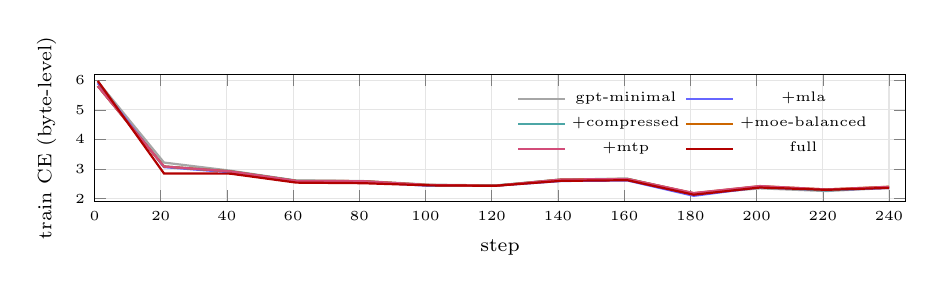
\begin{tikzpicture}
  \begin{axis}[
    width=0.98\columnwidth, height=3.2cm,
    xlabel={step}, ylabel={train CE (byte-level)},
    xmin=0, xmax=245, ymin=1.9, ymax=6.2,
    tick label style={font=\tiny}, label style={font=\scriptsize},
    legend style={font=\tiny, draw=none, fill=none, at={(0.97,0.95)}, anchor=north east}, legend columns=2,
    grid=major, grid style={gray!20},
  ]
  \addplot[gray!70, thick] coordinates {(1,5.952)(21,3.22)(41,2.947)(61,2.611)(81,2.597)(101,2.476)(121,2.446)(141,2.605)(161,2.648)(181,2.159)(201,2.35)(221,2.259)(240,2.364)};
  \addlegendentry{gpt-minimal}
  \addplot[blue!60, thick] coordinates {(1,5.897)(21,3.066)(41,2.893)(61,2.593)(81,2.575)(101,2.435)(121,2.439)(141,2.599)(161,2.615)(181,2.098)(201,2.389)(221,2.29)(240,2.365)};
  \addlegendentry{+mla}
  \addplot[teal!70, thick] coordinates {(1,5.803)(21,3.089)(41,2.925)(61,2.608)(81,2.589)(101,2.45)(121,2.444)(141,2.649)(161,2.674)(181,2.172)(201,2.411)(221,2.279)(240,2.396)};
  \addlegendentry{+compressed}
  \addplot[orange!80!black, thick] coordinates {(1,5.803)(21,3.088)(41,2.923)(61,2.599)(81,2.593)(101,2.462)(121,2.436)(141,2.648)(161,2.668)(181,2.185)(201,2.423)(221,2.313)(240,2.404)};
  \addlegendentry{+moe-balanced}
  \addplot[purple!70, thick] coordinates {(1,5.803)(21,3.088)(41,2.923)(61,2.599)(81,2.593)(101,2.461)(121,2.435)(141,2.647)(161,2.665)(181,2.191)(201,2.427)(221,2.312)(240,2.4)};
  \addlegendentry{+mtp}
  \addplot[red!70!black, thick] coordinates {(1,5.974)(21,2.853)(41,2.846)(61,2.543)(81,2.524)(101,2.451)(121,2.436)(141,2.603)(161,2.624)(181,2.135)(201,2.378)(221,2.3)(240,2.365)};
  \addlegendentry{full}
  \end{axis}
  \end{tikzpicture}
  \caption{Training curves for the six presets of Table~\ref{tab:ladder}
  (identical data, optimizer, and seed; main next-token loss only, so the
  values are comparable across presets with and without auxiliary heads).}
  \label{fig:ladder-curves}
\end{figure}

\paragraph{Serving throughput by cohort size.} End-to-end decode throughput
(prefill included) on the machine of Table~\ref{tab:ladder}, complementing
Figure~\ref{fig:batching}: 316, 546, 810, and 1{,}389 aggregate tok/s at
cohort sizes 1, 2, 4, and 8 ($1.0\times$, $1.7\times$, $2.6\times$,
$4.4\times$).

\paragraph{Bits-per-byte across the lineage.} The full matrix behind the
capability column of Table~\ref{tab:biography} (150 blocks per corpus;
know-nothing baseline 8.0 bpb):

\begin{table}[h]
\centering
\small
\begin{tabular}{@{}lcc@{}}
\toprule
Checkpoint & pre-train corpus & repository code \\
\midrule
pre-train & 3.151 (ppl 158.2) & 2.561 (ppl 165.2) \\
mid-train & 1.706 (ppl 15.5) & 1.153 (ppl 10.0) \\
\bottomrule
\end{tabular}
\caption{Bits-per-byte (and token perplexity) for the lineage's first two
stages. Repository code is unseen by the pre-train checkpoint; the mid-train
checkpoint trains on it, so its in-domain value is a fit measure while the
cross-domain column shows retained generality.}
\label{tab:bpb}
\end{table}

\paragraph{Speculative decoding, expected gain.} With $k$ drafted tokens and
per-token acceptance probability $p$, the expected tokens emitted per verify
pass is $(1-p^{k+1})/(1-p)$: for the course's $k{=}4$ configuration this is
$1.43$, $1.94$, $2.77$, and $4.10$ at $p \in \{0.3, 0.5, 0.7, 0.9\}$---up to
$4.1\times$ fewer forward passes than greedy decoding.

\paragraph{Reproducibility.} All measurements regenerate from committed
artifacts: \texttt{run\_experiments.py} (Table~\ref{tab:ladder},
Figure~\ref{fig:ladder-curves}),
\texttt{stage\_evals.json} (Tables~\ref{tab:biography} and~\ref{tab:bpb}),
and \texttt{pretrain\_reference.json} (Figure~\ref{fig:loss}). Following G3,
\texttt{verify\_claims.py} re-derives every countable statement of this
manuscript and exits non-zero on mismatch; all checks pass, and the script
runs in the repository's public CI.
